\chapter{Target Acquisition}%
\label{ch:target-acquisition}
An autonomous mobile robot must be able to navigate to a target
position. Information about the target position can be provided by \textit{a
  priori} knowledge of the target coordinates --- $\gls{xtar}, \gls{ytar}$ --- or the
robot computer vision system may indicate the direction of the target (see
Fig.~\ref{fig:fig1}).
%
% Fig 1
\begin{figure}[!hbt]
\centering
    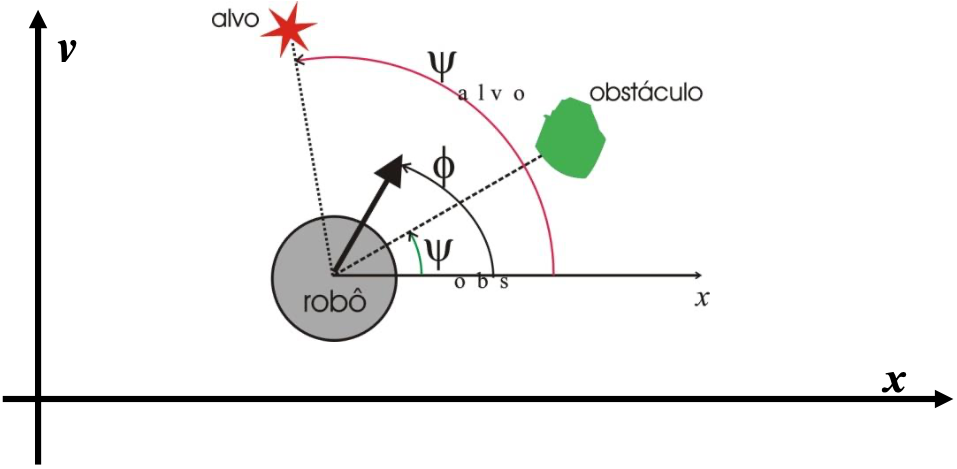
\includegraphics[width=0.6\textwidth]{./img/fig1.png}
  \caption[Target acquisition heading angle referencing to external world
  axes]{Target acquisition heading angle referencing to external world axes: The angle by which the robot `sees', $\gls{psi-tar}$, the target in
    relation to external world axes may be yielded by the robot's computer
    vision system or may be computed if the target coordinates ($x_{tar},
    y_{tar}$) are known and one has an estimative of the position of the robot
    ($x_{robot}, y_{robot}$)}%
\label{fig:fig1}
\end{figure}

The target acquisition behavior can be yielded by dynamic systems for the
heading direction and linear velocity:
%
\begin{equation}
  \label{eq:3}
  \frac{d \phi}{dt} = f_{tar}(\phi{,} \psi _{tar}) + f_{stoch}
\end{equation}
\begin{equation}
  \label{eq:4}
\frac{dv}{dt} = g_{tar} (v)
\end{equation}

The term $\gls{ftar}$ of the vectorial field in the equation~(\ref{eq:3}) may have
the nonlinear form:
\begin{equation}
  \label{eq:5}
f_{tar}(\phi{,} \psi _{tar}) = - \lambda _{tar} \sin (\phi - \psi _{tar})
\end{equation}
%
where $\gls{lambda-tar}$ is a parameter that defines the magnitude of the
`attraction force' the target exerts over the robot and $\psi _{tar}$ is the
direction the robot `sees' the target.

The term $\gls{fstoch}$ of the vectorial field in the equation~(\ref{eq:3})
represents the stochastic force that must be present to ensure escape from
repellers within a limited time:
\begin{equation}
  \label{eq:6}
f_{stoch} = \sqrt{Q} \varepsilon _{n}
\end{equation}
modelled as Gaussian white noise, $\gls{varepsilon-n}$, of unit variance, so that
$\gls{Q}$ is the effective variance of the force~\cite{bicho2000dynamic}.

\section{Analytical study of nonlinear dynamic system defined by
  Eqs. (\ref{eq:3}) and (\ref{eq:5})}%
\label{sec:analyt-study-tar-nonl}
In this section, an analytical study of the dynamic system defined by
Eqs. (\ref{eq:3}) and (\ref{eq:5}) is performed. The fixed points of this
dynamic system are determined and its stability is assessed, thus leading to
successfull positioning of the attractor for the heading direction. Then, the phase
portraits and bifurcation diagram are drawn, yielding the range of admissible
values for the magnitude of the attractor.

\subsection{Fixed points of the dynamic system}%
\label{sec:fixed-points-dynamic}
The fixed points of the dynamic system are the values, $\gls{phi-star}$, for which the
state of the system does not change, i.e., $f_{tar}(\phi^*) = 0$. Once placed at
a fixed point, the system remains fixed in that state ($d \phi / dt = 0$), hence
also named as constant solutions of the dynamic system. Graphically, the fixed
points correspond to the intersection of the function $f(\phi)$ with the $\phi$
axis.

Fig.~\ref{fig:1-1-fixed-points} illustrates the determination of the fixed
points of the dynamic system, given by Eq.~(\ref{eq:7}),yielding the general solution:
$\phi^* = \psi_{tar} + k \pi$. As the heading direction $\phi \in [0, 2 \pi[$
represents a circular phase space, the solutions can be limited to $\phi_1^* =
\psi_{tar}, \phi_2^* = \psi_{tar} + \pi$.
\begin{equation}
  \label{eq:7}
  \left. \frac{d \phi}{dt}\right|_{\phi = \phi^*} = f_{tar}(\phi^*) = 0
\end{equation}
% fixed points
\begin{figure}[!hbt]
\centering
    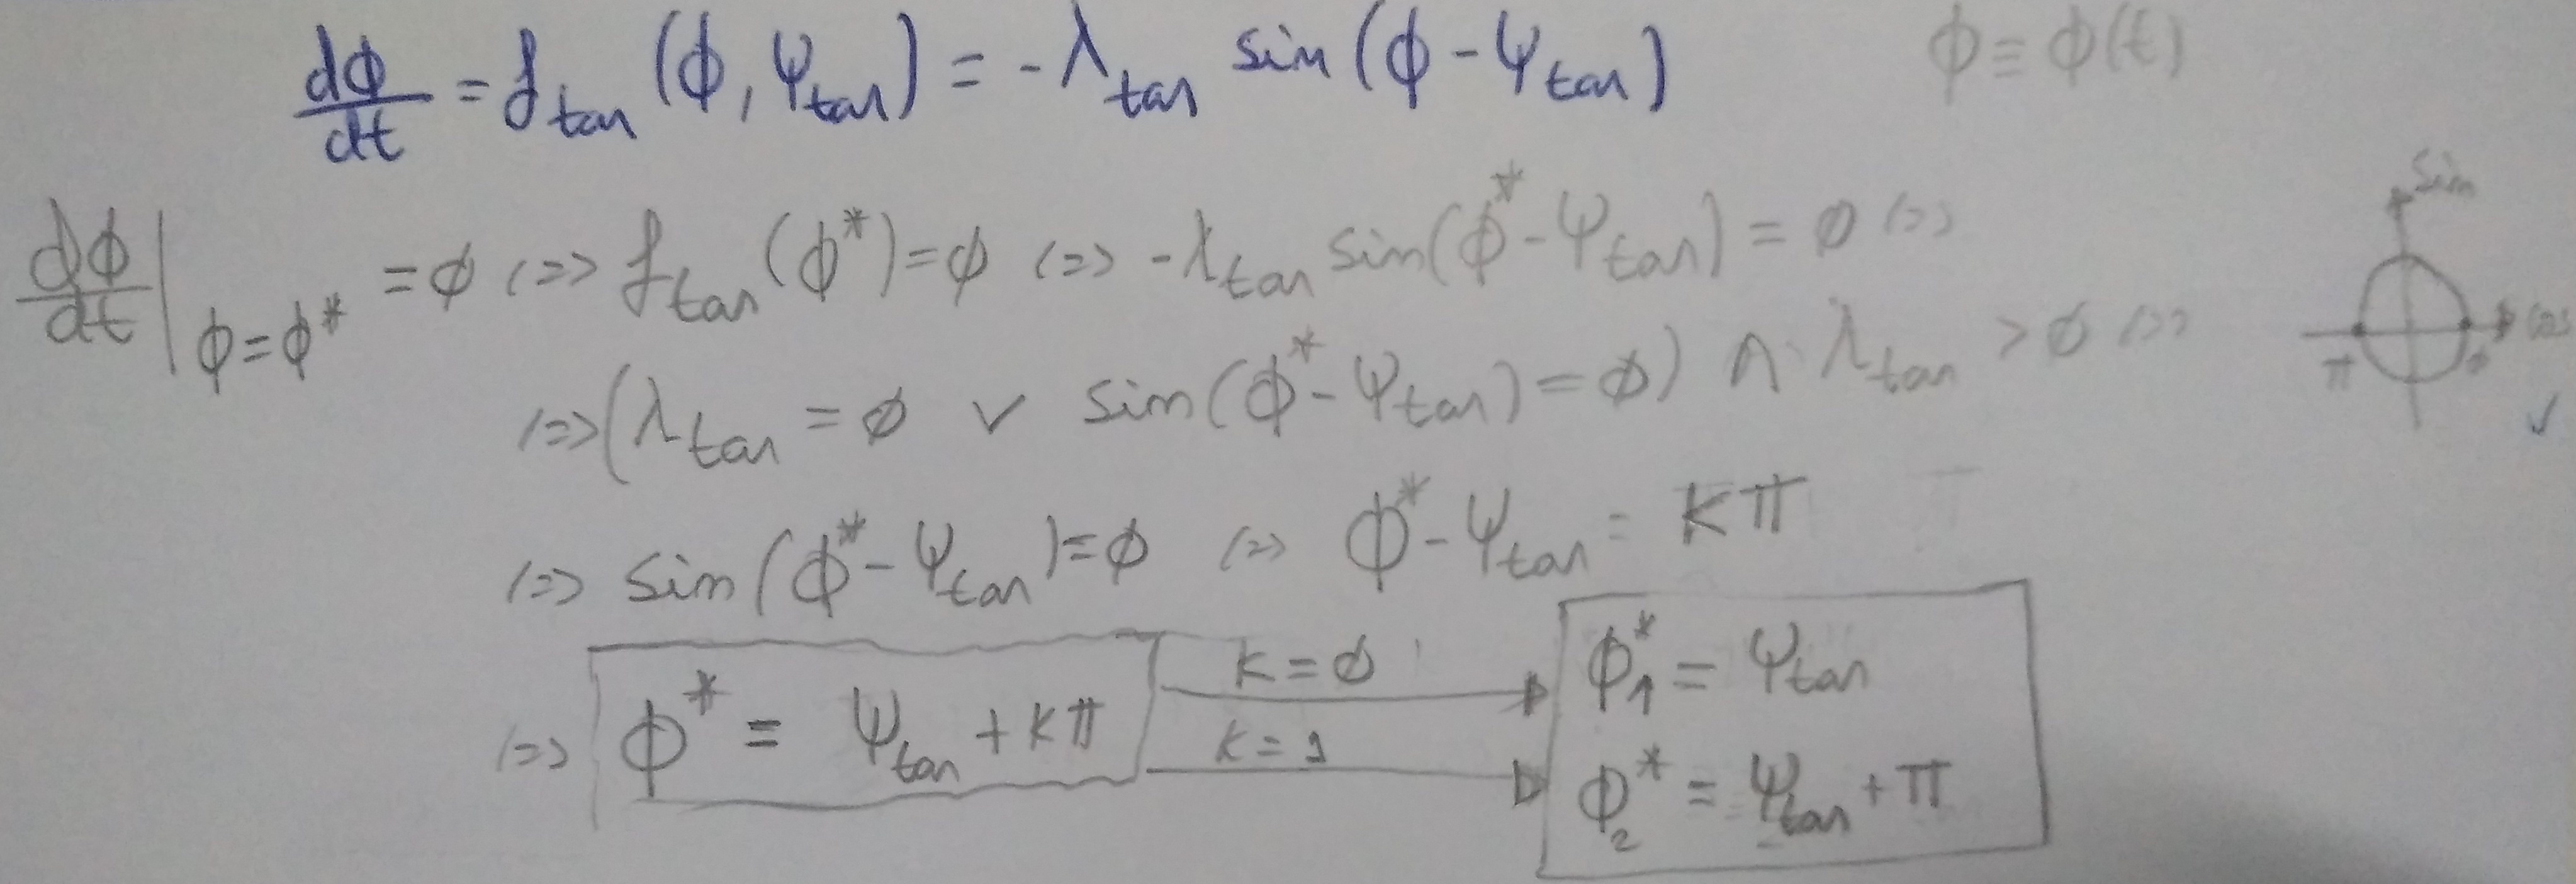
\includegraphics[width=1.0\textwidth]{./img/1-1-fixed-points.jpg}
  \caption{Target acquisition behavior: Determination of fixed points}%
\label{fig:1-1-fixed-points}
\end{figure}
% 
\subsection{Stability of the fixed points and relaxation time}%
\label{sec:stab-fixed-points}
The determination of the stability of fixed points is useful to understand its
qualitative behavior. It can be determined analytically using Eq.~(\ref{eq:8}),
or infered graphically by observing the slope of $f_{tar}(\phi)$ at the fixed
points.
%
\begin{equation}
  \label{eq:8}
  m = \left. \frac{d f_{tar}(\phi)}{d \phi}\right|_{\phi = \phi^*}
\end{equation}

Three cases arise, depending on the sign of $\gls{m}$:
\begin{enumerate}
\item $m < 0$: $\phi^*$ is an asymptotically stable state, i.e., an attractor;
\item $m > 0$: $\phi^*$ is an unstable state, i.e., an repeller;
\item $m = 0$: nothing can be concluded about $\phi^*$ using the analytical
  method. The graphical method must be used.
\end{enumerate}

The relaxation time, $\gls{tau-tar}$, corresponds to the required time for the system state be
significantly attracted to the asymptotically stable state when it is in the
vicinity of this fixed point. It can be determined from the inverse of the slope
on the vicinity of the fixed point, as given by Eq.~(\ref{eq:9}):
\begin{equation}
  \label{eq:9}
  \tau_{tar} = \frac{1}{| f'(\phi^*) |}
\end{equation}

Fig.~\ref{fig:1-2-stability-fixed-points} illustrates the assessment of the
stability of the fixed points and the relaxation time. It can be observed that
the analytical method provides $m_1 = - \lambda_{tar}, m_2 = \lambda_{tar}$.
Thus, for the attractor to be placed in the target direction, i.e. $\phi_1^* =
\psi_{tar}$, and an repeller in the opposite direction, i.e., $\phi_2^* =
\psi_{tar} + \pi$ as expected, $\lambda_{tar} > 0$.
This way the robot can rapidly divert from the repeller and move to the
attractor direction. The relaxation time is inversely proportional to the local
time constant, i.e., inversely proportional to the magnitude of the attractive
force-let $\tau_{tar} = 1/\lambda_{tar}$ s.
%
% stability
\begin{figure}[!hbt]
\centering
    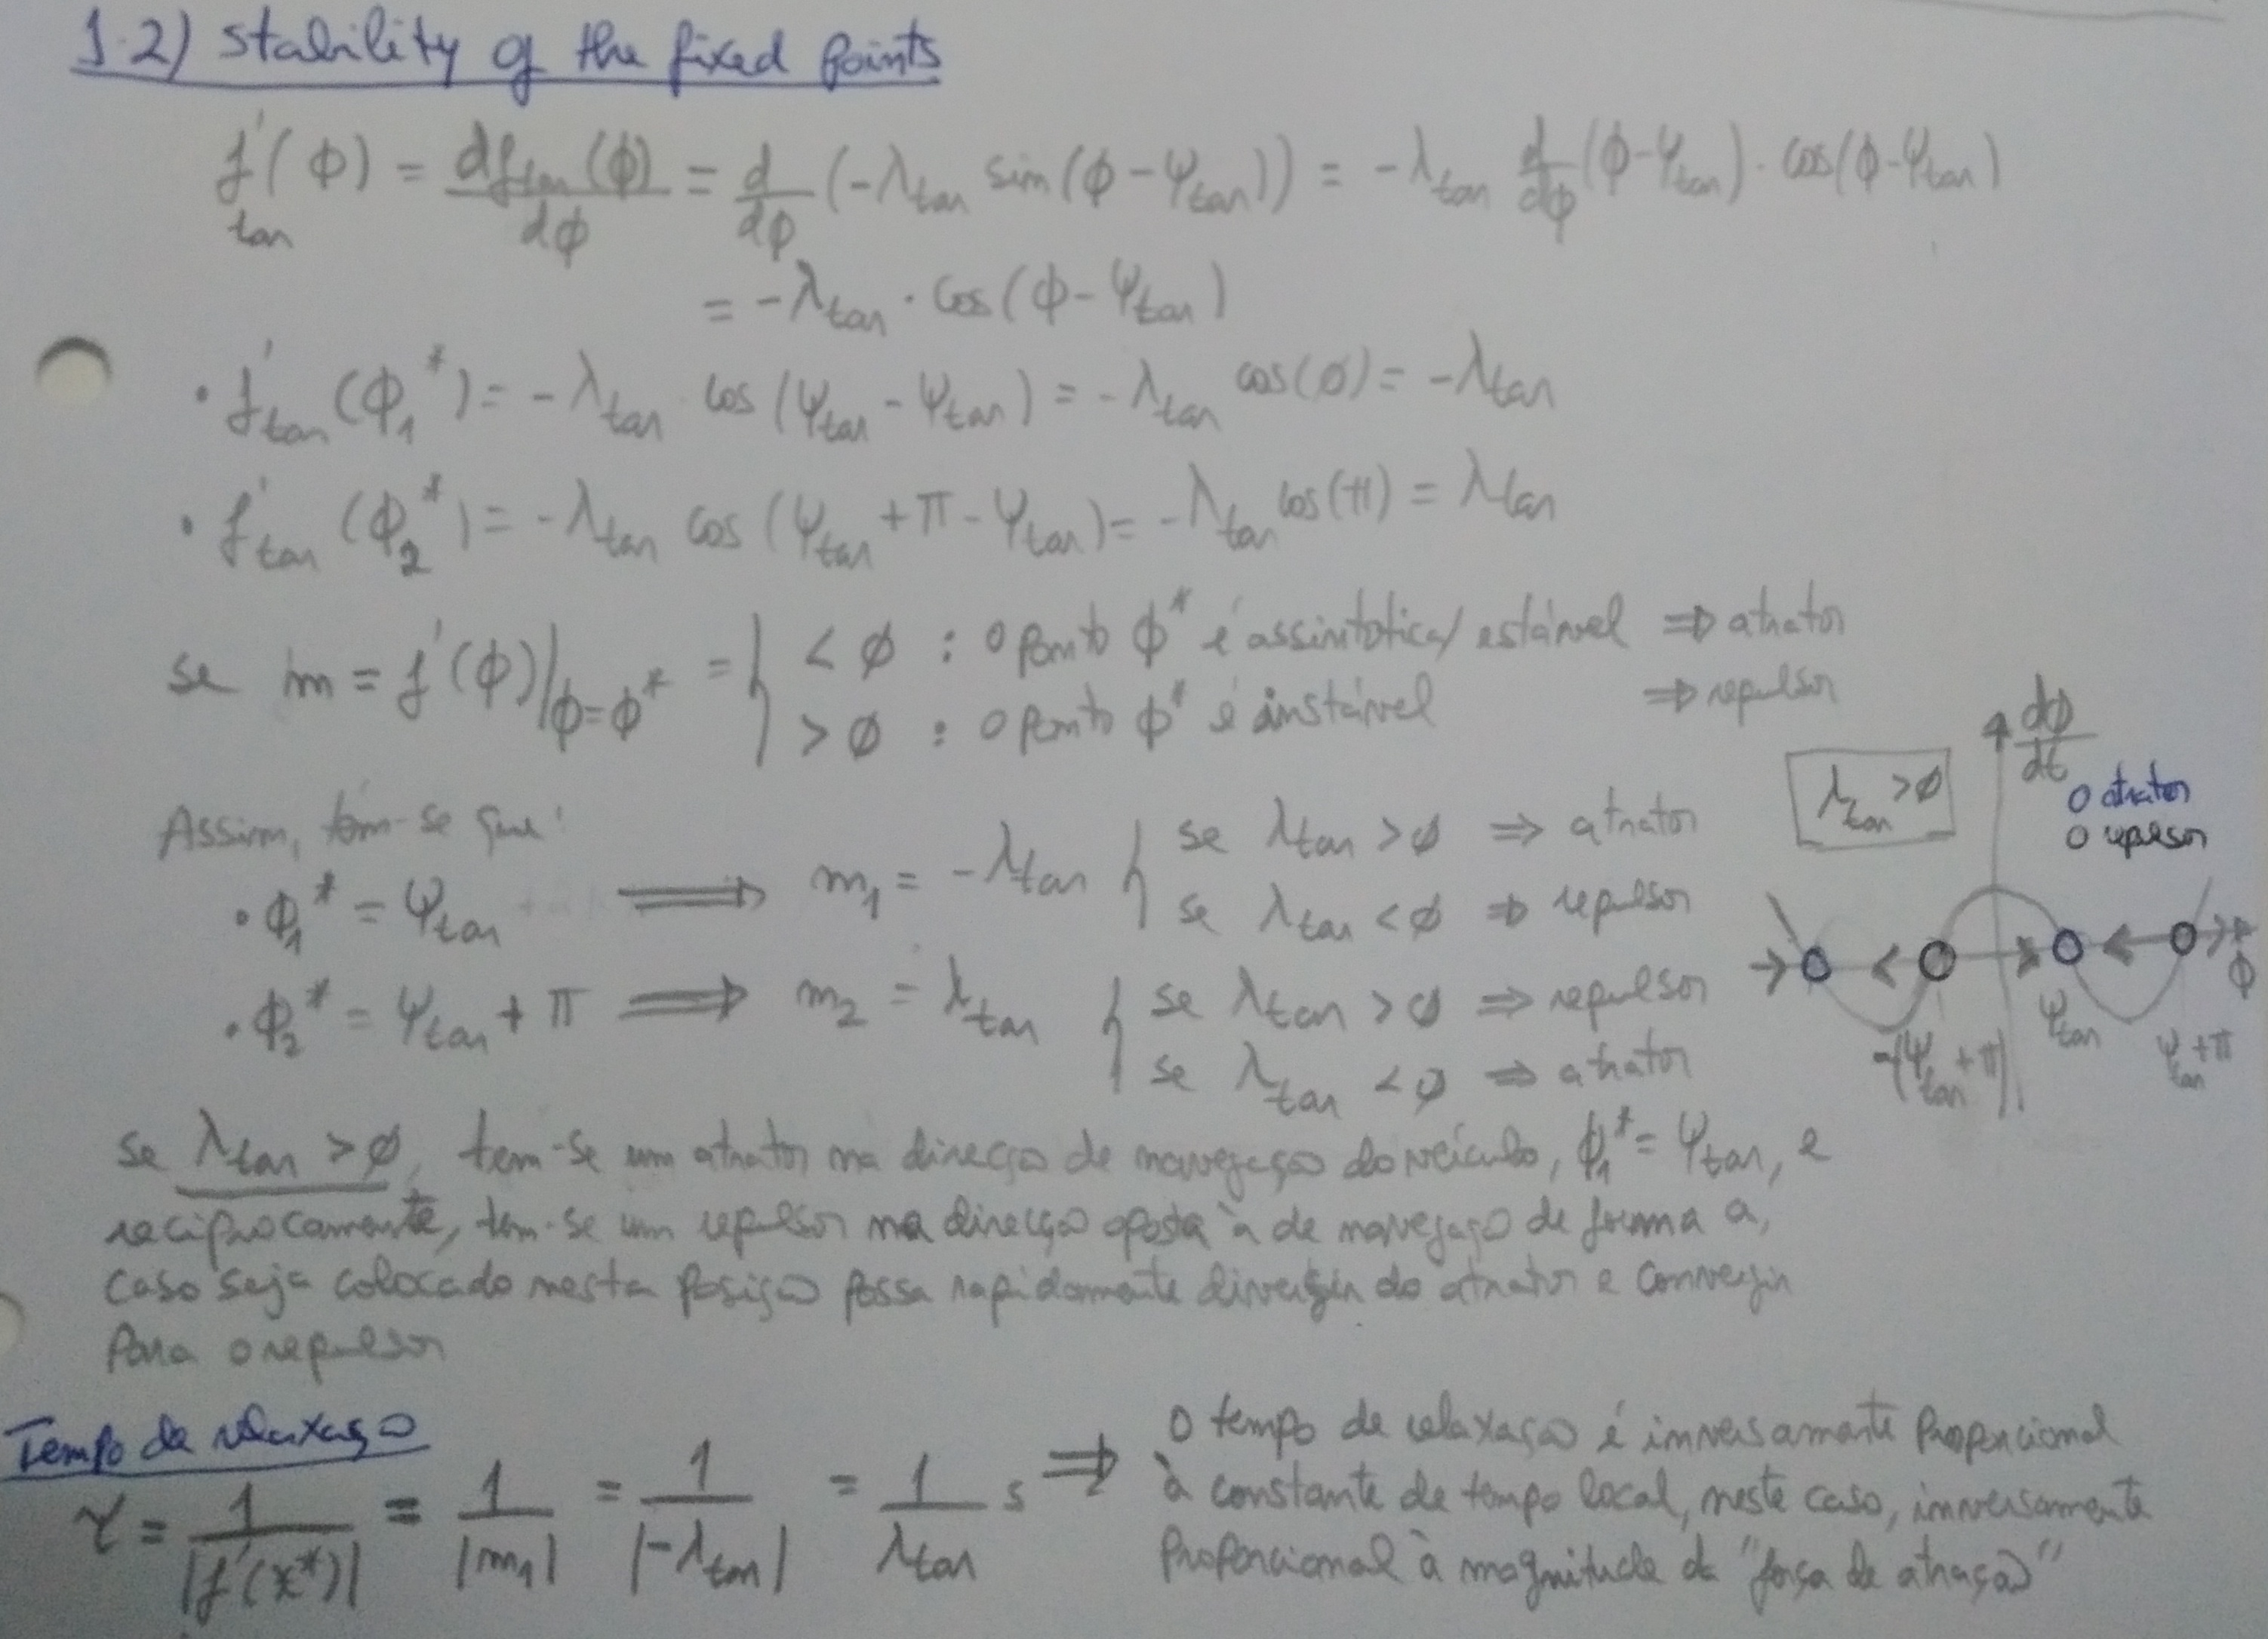
\includegraphics[width=1.0\textwidth]{./img/1-2-stability-fixed-points.jpg}
  \caption{Target acquisition behavior: Stability of fixed points and relaxation time of the attractor}%
\label{fig:1-2-stability-fixed-points}
\end{figure}
%
\subsection{Phase portraits}%
\label{sec:phase-portraits}
The phase portrait of a dynamic system consists in a graphical representation
that shows all its qualitatively different trajectories. The fixed points are
represented as circles and the evolution direction of the state $\phi$ as the
time progresses is indicated by arrows --- convergent arrows to attractors and
divergent arrows from repellers.

Fig.~\ref{fig:1-3-phase-portraits} depicts the possible phase portraits for the
target acquisition dynamic system, depending on the sign of the parameter
$\lambda_{tar}$:
\begin{itemize}
\item $\lambda_{tar} > 0$: an attractor is placed in the target direction and a
  repeller is placed in the opposite direction. This represents the intended
  behavior for the system.
\item $\lambda_{tar} < 0$: a repeller is placed in the target direction and a
  attractor is placed in the opposite direction. This represents an undesired
  behavior for the system.
\end{itemize}
%
% phase-portraits
\begin{figure}[!hbt]
\centering
    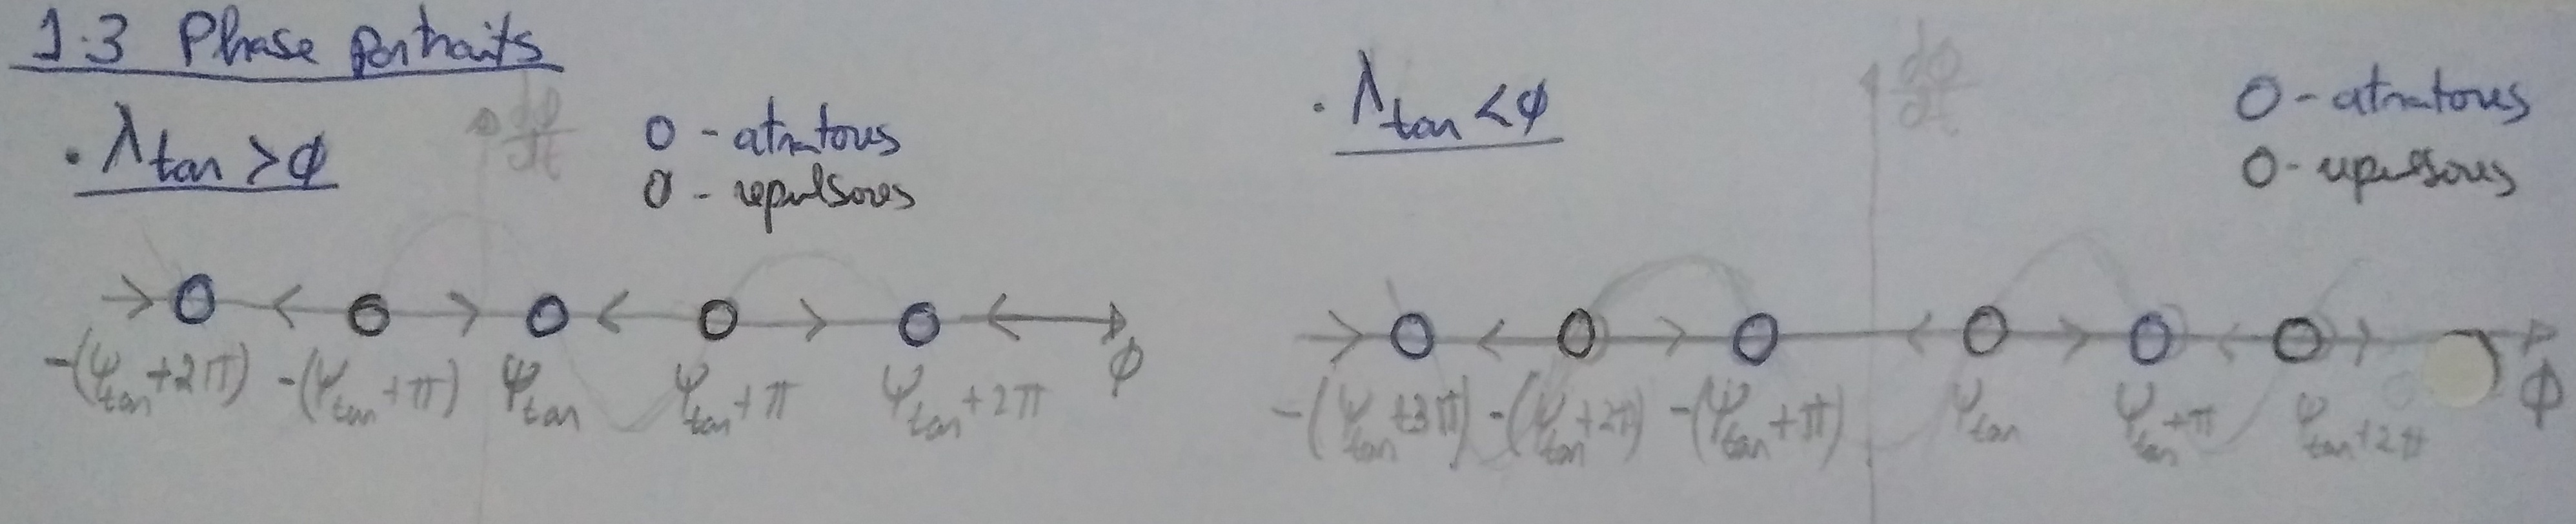
\includegraphics[width=1.0\textwidth]{./img/1-3-phase-portraits.jpg}
  \caption{Target acquisition behavior: Phase portraits}%
\label{fig:1-3-phase-portraits}
\end{figure}
%
\subsection{Bifurcation diagram}%
\label{sec:bifurcation-diagram}
Bifurcations arise as the qualitative behavior of the system changes, i.e., the
number, nature and/or stability of the fixed points changes. A bifurcation point
is the value of the parameter for which the qualitative change of the system
behavior occurs. The bifurcation diagram consists in a graphical representation
of the fixed points and respective stability as a function of a parameter of
$f(\phi)$.

Fig.~\ref{fig:1-4-bifurcation-diag} depicts the bifurcation diagram for the
target acquisition dynamic system, as a function of the parameter $\lambda_{tar}$
for both fixed points --- $\phi_1^* = \psi_{tar}, \phi_2^* = \psi_{tar} - \pi,
\psi_{tar} > 0$:
\begin{itemize}
\item $\lambda_{tar} < 0$: the fixed point $\phi_1^*$ is unstable and
  $\phi_2^*$ is asymptotically stable.
\item $\lambda_{tar} > 0$: the fixed point $\phi_1^*$ becomes asymptotically stable and $\phi_2^*$ is unstable.
\end{itemize}
%
$\lambda_{tar} = 0$ is a bifurcation point. This represents a transcritical bifurcation as there is an exchange in the
stability between fixed points.
%
% Bifurcation diagram
\begin{figure}[!hbt]
\centering
    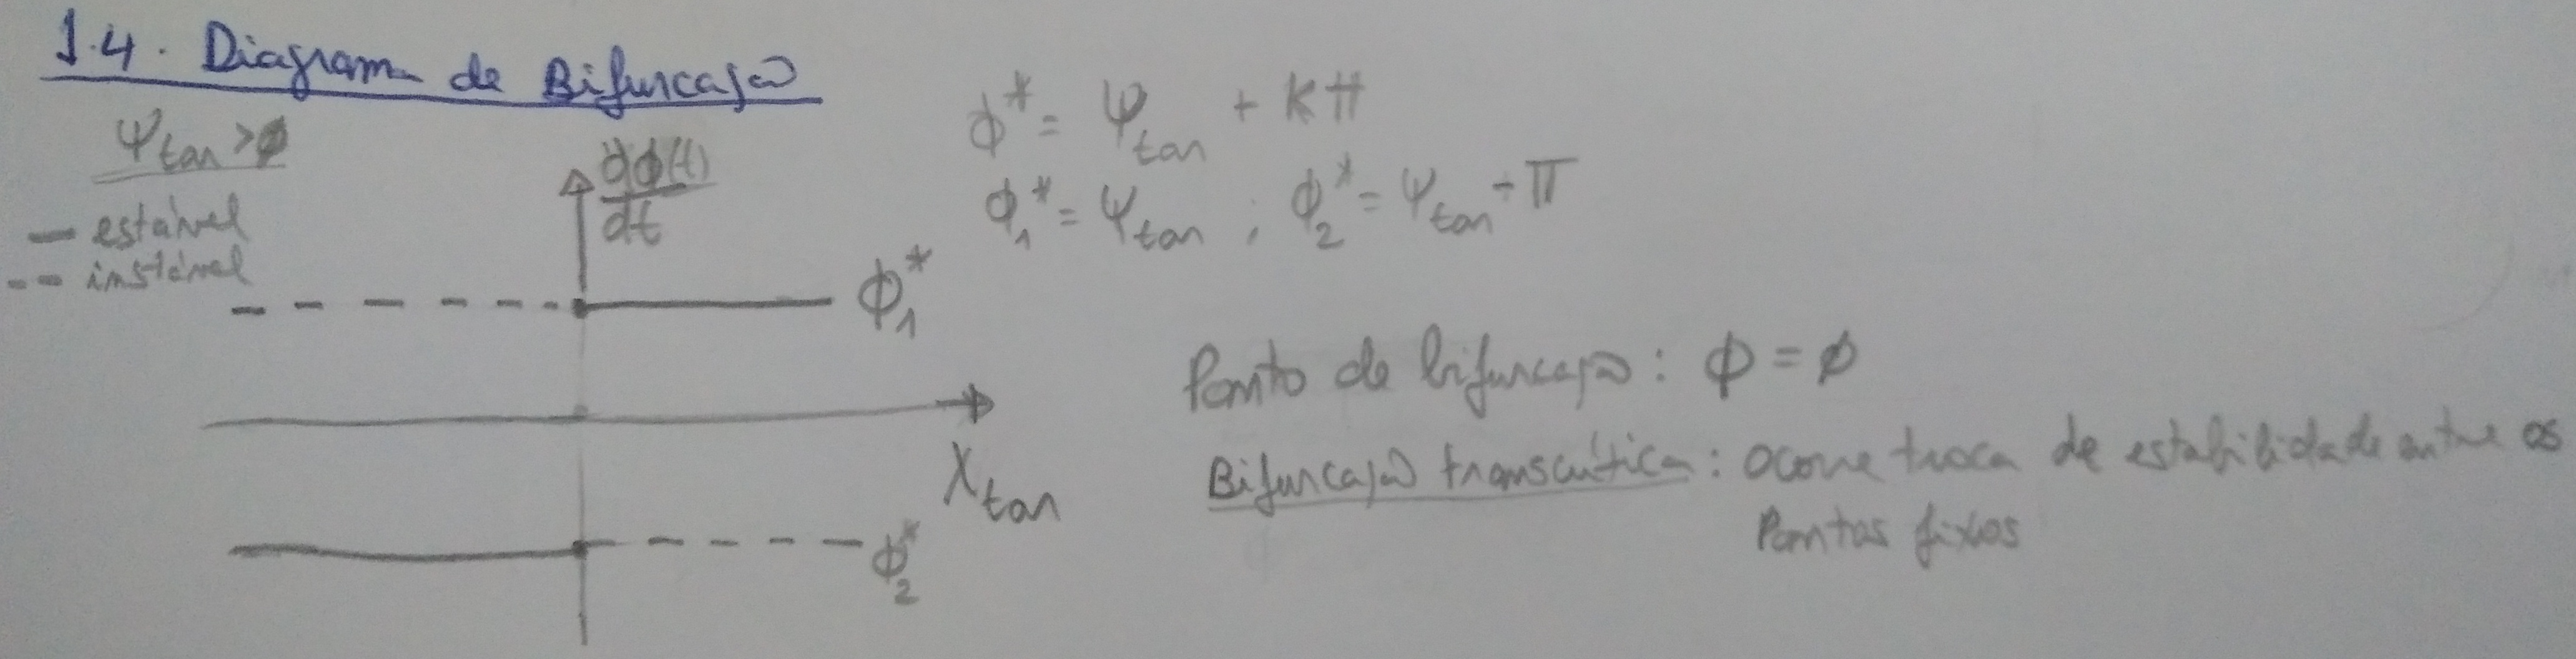
\includegraphics[width=1.0\textwidth]{./img/1-4-bifurcation.jpg}
  \caption{Target acquisition behavior: Bifurcation diagram}%
\label{fig:1-4-bifurcation-diag}
\end{figure}
%
\subsection{Range of values for $\lambda _{tar}$}%
\label{sec:range-tar}
For the target acquisition behavior, i.e. for the robot to move the target, an
attractor must be placed in the direction of the target, thus $\phi_1^* =
\psi_{tar}$ must be an asymptotically stable state of the system and consequently $\lambda_{tar} > 0$. 
\section{Implementation of nonlinear dynamic system defined by
  Eqs. (\ref{eq:3}) and (\ref{eq:5})}%
\label{sec:implem-study-tar-nonl}
In this section is demonstrated the implementation of the nonlinear dynamic
system for the heading direction. Additionally, a linear dynamic system for
the linear velocity of the robot is also implemented.

The first step of the implementation is to convert the first order differential
equation into an algebraic recursive equation by applying the forward Euler's
method in a discrete form:
\begin{equation}
  \label{eq:10}
  \phi(t + \Delta t) = \phi(t) + \Delta t f(\phi), \qquad \phi(t_0) = \phi_0
\end{equation}
where $\gls{delta-t}$ is the Euler's step --- the incremental timestep applied to
the recursive equation. For smooth variation of the heading direction the
Euler's step must be significantly smaller than the minimum time constant (in
this case, the relaxation time), i.e.: $\Delta t \ll \tau _{tar}$. As a rule of
thumb: $5 \Delta t \le \tau_{tar} \le 10 \Delta t$.

Next, the direction of the target, $psi_{tar}$ must be determined, based on the
known target coordinates and the robot's estimated coordinates with respect to
the external reference axis, respectively, $(x_{tar},y_{tar})$ and $(\gls{xrobot},
\gls{yrobot})$, taking into consideration the quadrant, as follows (see Fig.~\ref{fig:fig1}):
\begin{equation}
  \label{eq:11}
 \psi_{tar} = atan2 \Big(\frac{y_{tar} - y_{robot}}{x_{tar} - x_{robot}}\Big)
\end{equation}
It is important to note that the target acquisition dynamics is dependent
on the calibration of the heading direction of the robot in respect to the
external reference axis to accurately locate it.

Then, both components of the dynamic system, $f_{tar}$ and $f_{stoch}$ can be
computed using Eqs.~(\ref{eq:5}) and~(\ref{eq:6}) and added, yielding the
complete dynamic system as given by Eq.~(\ref{eq:3}). Next, the angular velocity
of the vehicle can be determined, noting that $\omega _{robot} = d \phi /dt$,
i.e., equal to the complete vector field.

Finally, linear velocity is defined, and, if desired a stop criterion for the
distance to target. Then, the values of the angular and linear velocities of the
robot can be passed as setpoints to the low-level code responsible for
controlling these control variables.

Summarizing, the pseudocode for the target acquisition behavior is as follows:
\begin{enumerate}
\item Initialize robot: retrieve simulation timestep and robot characteristics
\item Set initial values (linear and angular velocities) and set robot's initial
  pose ($x_{robot}, y_{robot}, \phi_{robot}$)
\item Initialize target
\item While target <= targetNr
  \begin{enumerate}
  \item Exchange information with the simulator
  \item Get vehicle's pose, target position and simulation timestep
  \item Trigger a simulation step
  \item Processing step
    \begin{enumerate}
    \item Set parameters values: $\tau_{tar}, \lambda_{tar}, Q$
    \item Compute $\psi_{tar}$
    \item Compute $f_{tar}$ and $f_{stoch}$
    \item Compute resultant vector field $f_{total}$ and assign it to angular
      velocity
    \item Set linear velocity
    \item Define stop criterion for target distance (if desired)
    \end{enumerate}
  \item View dynamics: plot the target acquisition dynamics
  \item Set robot's angular and linear velocities
  \end{enumerate}
\item Terminate simulation and cleanup
\end{enumerate}

As a result, the following generic Matlab code was implemented (Listing~\ref{lst:program-dyn-tar}):
% program_dyn_tar.m (generic)
\lstinputlisting[language=matlab, caption={Generic implementation of target
  acquisition behavior (not tuned)},label=lst:program-dyn-tar,
style=custom-matlab]{./listing/program_dyn_tar.m}%

Several scenarios have been simulated in CoppeliaSim/Matlab --- scenario
\texttt{MobileRobotDyn\_tar.ttt} --- for different linear velocity conditions namely:
\begin{enumerate}
\item Robot with rotational motion only: v = 0 m/s;
\item Robot moving at constant speed: v = K m/s;
\item Robot moving at a velocity defined by a vectorial field;
\end{enumerate}
%
\subsection{Rotational motion only}%
\label{sec:robot-initially-at}
In this first scenario, one considers only the existence of the rotational
motion of the robot in respect to its center of mass, i.e., v = 0 m/s. The
parameters were tuned to guide the robot for the desired target direction.

The scenario \texttt{MobileRobotDyn\_tar.ttt} was loaded in CoppeliaSim and the
robot was placed in the opposite direction of the target (worst case scenario),
as illustrated in Fig.~\ref{fig:tar-2-1-arena}. Then, the initial values of angular
and linear velocities were set and the parameters were tuned as indicated in
Listing~\ref{lst:program-dyn-tar-2-1}:
\begin{itemize}
\item $v_{robot} = 0$: robot does not exhibit translational motion.
\item $\tau_{tar} = 5 \Delta t$: minimum value to ensure forward Euler's method convergence.
\item $Q = 0.01$: sufficient effective variance of the Gaussian white noise to
  enable qualitative differences in the behavior (turn left/right).
\end{itemize}
% program_dyn_tar.m (generic)
\lstinputlisting[language=matlab, caption={Target acquisition behavior: Parameter tuning for v = 0 m/s},label=lst:program-dyn-tar-2-1,
style=custom-matlab]{./listing/program_dyn_tar_2_1.m}%

Fig.~\ref{fig:tar-2-1} illustrates the target acquisition dynamics in the final
condition. Initially, the heading direction, $\phi$, sits in a repeller $\phi =
50 + 180 ^{\circ}$ (positive slope). The heading direction diverts from this fixed point as it
represents an unstable state and tries to redirect to the attractor (turning in
clockwise direction) located at
$\phi = 50 ^{\circ}$ (negative slope). When it reaches this asymptotically
stable state the robot remains there, as intended. This validates the behavior
of orientation to the target.

Additionally, it is important to note the effect of the stochastic force: in
some occasions the robot follows a different trajectory for target orientation
by turning in counter-clockwise direction, depending on the randomized value of
the Gaussian white noise, $\varepsilon_n$.
%
\begin{figure}[!hbt]
\centering
    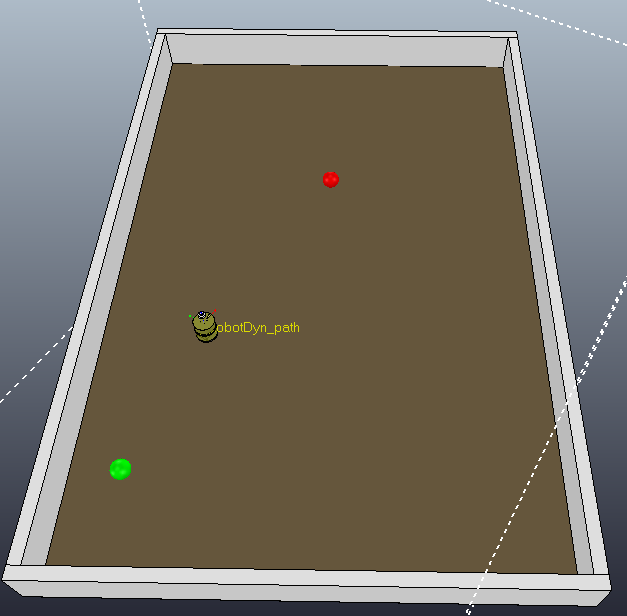
\includegraphics[width=0.7\textwidth]{./img/tar-2-1-arena.png}
  \caption{Target acquisition behavior: Simulation in CoppeliaSim for v = 0 m/s}%
\label{fig:tar-2-1-arena}
\end{figure}
%
\begin{figure}[!hbt]
\centering
    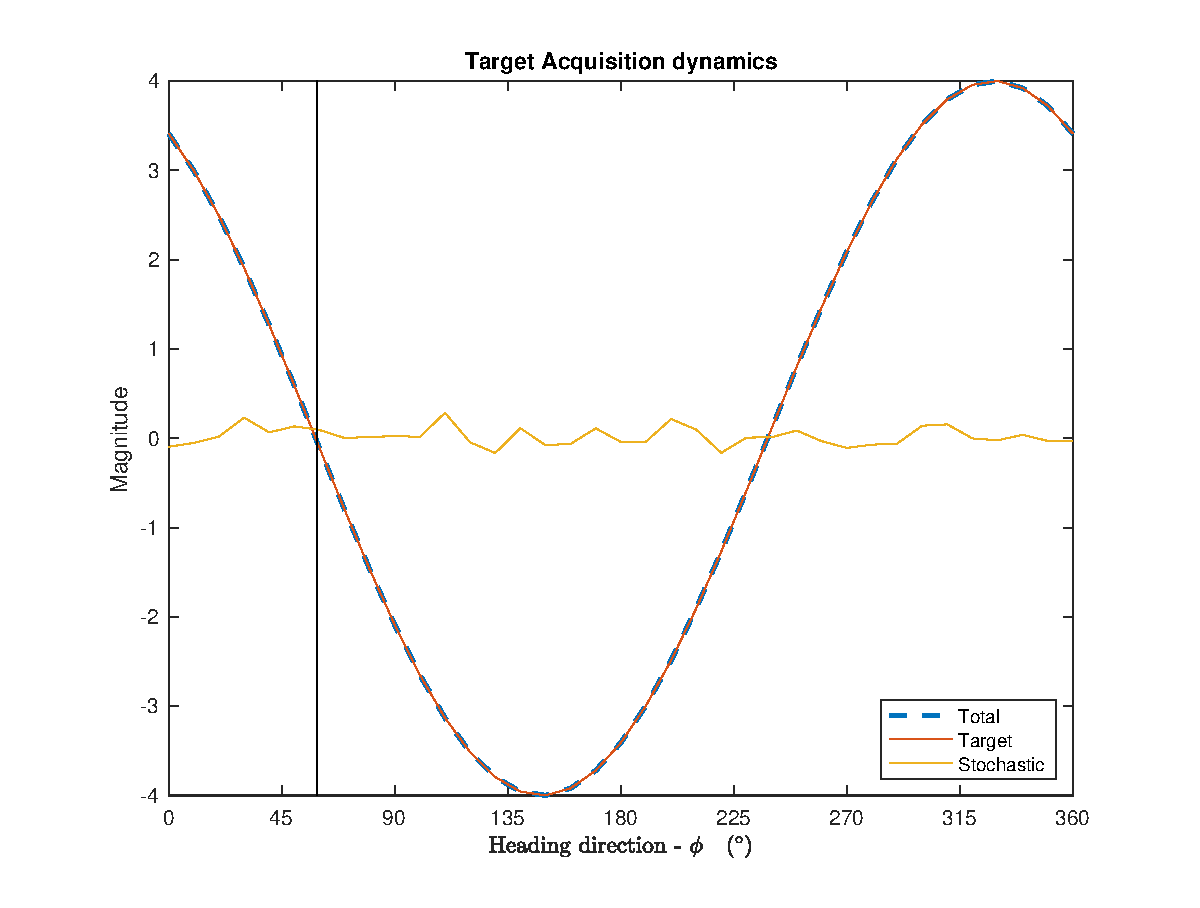
\includegraphics[width=0.6\textwidth]{./img/tar-2-1.eps}
  \caption{Target acquisition behavior: dynamics for v = 0 m/s}%
\label{fig:tar-2-1}
\end{figure}
%
\subsection{Robot moving at constant speed: v = K}%
\label{sec:robot-constant-speed}
After validating the behavior of orientation to the target, it is time to
implement the actual movement to the target by making the linear velocity $v
\neq 0$ m/s. First off, the linear velocity was set to a constant value and the
parameters were tuned, as illustrated in Listing~\ref{lst:program-dyn-tar-2-2},
where the only relevant change in respect to
Section~\ref{sec:robot-initially-at} is the value of the linear velocity.

Fig.~\ref{fig:tar-2-2-arena} depicts the simulation performed for $v = 30$
cm/s. The orientation behavior remains the same, but now the robot moves to the
desired target location (see also Video
\href{run:./videos/tar-2-2.mp4}{./videos/tar-2-2.mp4}), eventually colliding
with it at that speed, as no stop criterion is defined and the linear velocity
is independent from the distance to the target.
Increasing the linear
velocity of the vehicle increases the turning radius, slowing down the
orientation to the target. If the velocity is set too high and the vehicle is
close enough to the arena walls, it may crash against it before even turning (or
while turning).

The dynamics remains identical to the one in
Section~\ref{sec:robot-initially-at} (see Fig.~\ref{fig:tar-2-1}), although
slightly slower due to the increased turning radius for target orientation.
% program_dyn_tar.m (generic)
\lstinputlisting[language=matlab, caption={Target acquisition behavior: Parameter tuning for v = 30 cm/s},label=lst:program-dyn-tar-2-2,
style=custom-matlab]{./listing/program_dyn_tar_2_2.m}%
%
\begin{figure}[!hbt]
\centering
    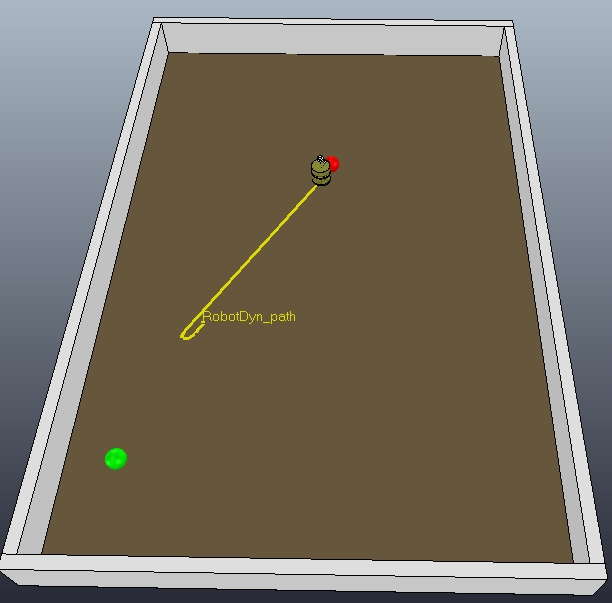
\includegraphics[width=0.7\textwidth]{./img/tar-2-2-arena.png}
  \caption{Target acquisition behavior: Simulation in CoppeliaSim for v = 30 cm/s}%
\label{fig:tar-2-2-arena}
\end{figure}
%
%
\subsection{Robot moving at a velocity defined by a vectorial field}%
\label{sec:robot-moving-vect-field}
Previously, the orientation and movement to the target were validated. However,
the linear velocity of the vehicle was constant and independent of the distance
to the target, which can be problematic especially if the velocity is high or a
stop criterion is undefined.

In this section a linear vectorial field is defined for the linear velocity of
the robot as given by Eq.~(\ref{eq:12}):
%
\begin{equation}
  \label{eq:12}
\frac{dv}{dt} = g_{tar} (v) = \lambda_v (v - v_{des})
\end{equation}
%
where $\gls{v-des}$ is the desired velocity and depends on the distance to the
target.

First, an analytical study of the vectorial field was performed for the
determination of its fixed points and respective stability --- similar to the
one in Section~\ref{sec:analyt-study-tar-nonl} ---  and the phase
portraits and bifurcation diagram were plotted (see
Fig.~\ref{fig:2-3-velocity-vectorial-field}). There is a fixed point at the
desired velocity, i.e., $\gls{v-star} = v_{des}$, which is asymptotically stable (an
attractor) if and only if $\gls{lambda-v} < 0$, yielding the intended
behavior. Additionally, the relaxation time to the attractor is given by
Eq.~(\ref{eq:9}), yielding $\gls{tau-v} = 1 / |\lambda_v| $.
%
\begin{figure}[!hbt]
\centering
    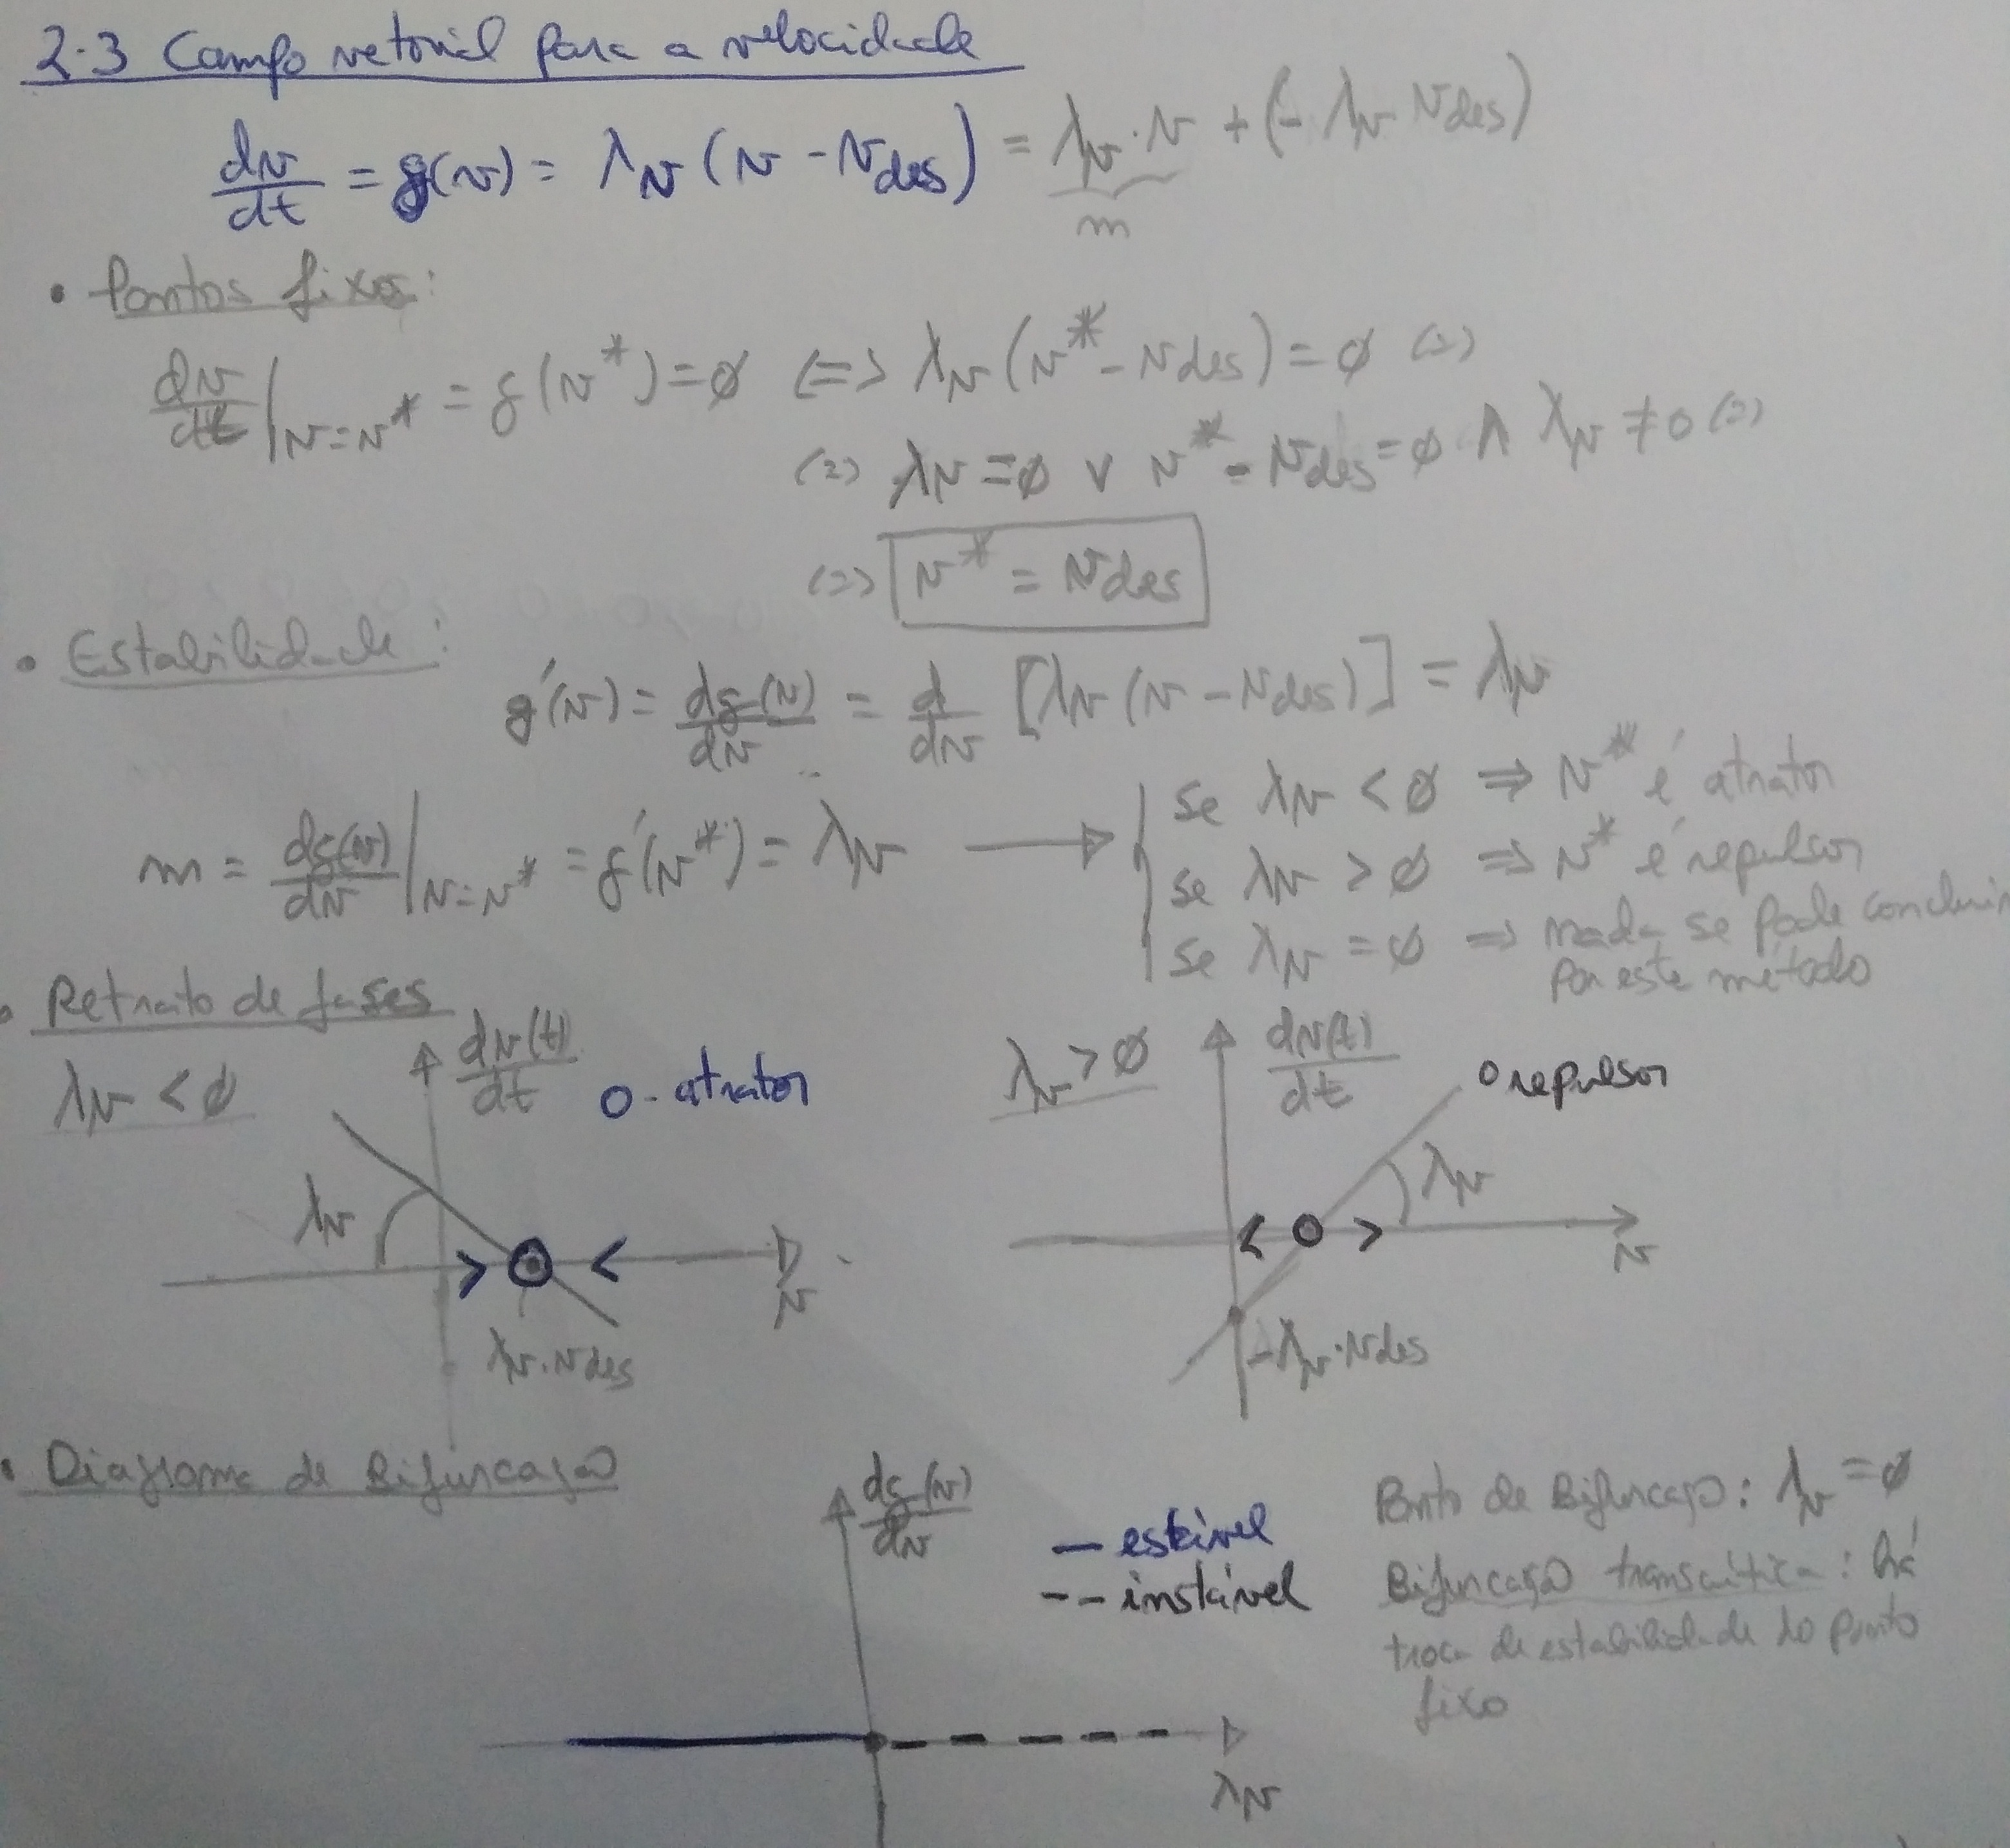
\includegraphics[width=\textwidth]{./img/2-3-velocity-vectorial-field.jpg}
  \caption{Target acquisition behavior: determination of the velocity dynamics}%
\label{fig:2-3-velocity-vectorial-field}
\end{figure}
%

The next step is to convert the first order differential equation into a
algebraic recursive equation in a discrete form (Eq.~(\ref{eq:13})):
\begin{equation}
  \label{eq:13}
v(t + \Delta t) = v(t) + \Delta t g_{tar}(v), \qquad v(t_0) = v_0
\end{equation}

Noting that $g_{tar}(v) = d v(t)/dt = a(t)$, one can write:
\begin{equation}
  \label{eq:15}
v(t + \Delta t) = v(t) + \Delta t a(t), \qquad v(t_0) = v_0
\end{equation}
which represents the equation of the uniformly varied rectilinear motion, with
$\gls{a}(t)$ being the acceleration of the robot. If $a(t) > 0$ the motion is
accelerated and reciprocally if $a(t) < 0$ the motion is retarded. Thus, one can
analyse the sign of $a(t)$ to understand the motion of the robot. Recalling that
$\lambda_v < 0$:
%
\begin{equation}
  \label{eq:16}
a(t) = g(v) = \left\{
\begin{array}{ll}
      > 0 , & (v - v_{des}) \leq 0 \\
      < 0 , & (v - v_{des}) > 0 \\
\end{array} 
\right. \leftrightarrow a(t) = g(v) = \left\{
\begin{array}{ll}
      > 0 , & v \leq v_{des} \\
      < 0 , & v > v_{des} \\
\end{array} 
\right. 
\end{equation}
%
the motion will be accelerated if $v \leq v_{des}$ --- which represents the
initial condition, ramping from rest to the desired velocity --- and retarded if
$v > v_{des}$ --- the inertia and delayed actuation (as a consequence of the
timestep) may lead to excessive velocity. On the other hand, the linear velocity
should converge to a constant value in the vicinity of the desired velocity
($a(t) = 0 \rightarrow v(t + \Delta t) = v(t)$).
%\begin{equation*}
%\frac{\Delta v}{\Delta t} = \lambda_v (v - v_{des}) \quad \leftrightarrow \quad v(t + \Delta t) - v(t) = \Delta t \lambda_v (v(t) - v_{des})
%\end{equation*}
%Rearraging the terms, the algebraic recursive equation for the linear velocity
%dynamic system becomes:
%\begin{equation}
%  \label{eq:13}
%v(t + \Delta t) = v(t) ( 1 + \Delta t \lambda_v) +  \Delta t \lambda_v v_{des}
%\end{equation}

With this in mind, one must determine the desired velocity as a function of the
distance to the target. Ideally, one desires a steady increase of velocity with
the distance and a plateau for the maximum velocity, which can be expressed as:
%
\begin{equation}
  \label{eq:14}
  v_{des} (d) = v_{max} - v_{max} e^{- \frac{d}{\tau_{vdes}}} \quad
  \leftrightarrow \quad
  v_{des} (d) = v_{max} \Big (1 - e^{- \frac{d}{\tau_{vdes}}} \Big )
\end{equation}
where $\gls{vmax}$ is the maximum velocity (cm/s) and $\gls{tau-vdes}$ is the time
constant for the desired velocity increase.

Fig.~\ref{fig:linear-vel-funcs-comparison} illustrates a comparison of
functions for the desired velocity as a function of distance, $v_{des}(d)$. The
maximum velocity considered was 80 cm/s.
The dashed line corresponds to the linear function $v_{des}(d) = \gls{kv} d$, with $k
= 1$, which acts as a guideline, although it could also be used, provided the
$v_{max}$ threshold was defined. For $\tau_{vdes} \leq 20$ s, the robot would hit the
target fast, which can be problematic due to path corners and
inertia; for $\tau_{vdes} \ge 75$ s it can be
slow. A tradeoff between velocity and path smoothness must be considered, as
detailed further ahead.     
%
\begin{figure}[!hbt]
\centering
    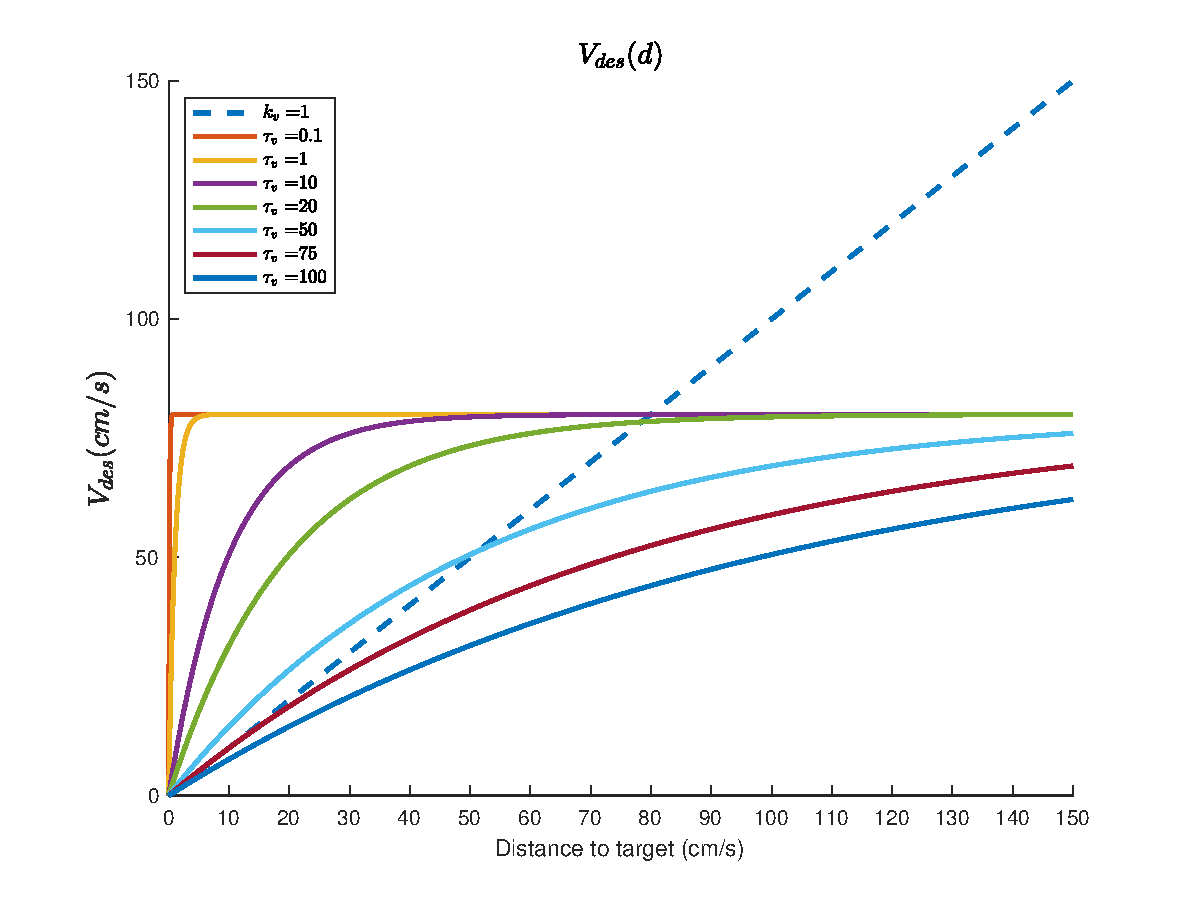
\includegraphics[width=0.7\textwidth]{./img/linear-vel-funcs-comparison.eps}
  \caption{Target acquisition behavior: comparison of functions $v_{des} (d)$}%
\label{fig:linear-vel-funcs-comparison}
\end{figure}

Lastly, the distance to the target, $gls{d}$, must be determined. It can be seen from
Fig.~\ref{fig:fig1} the distance to the target is given by the
euclidean distance in the cartesian plane, i.e.:
\begin{equation}
  \label{eq:17}
  d = \sqrt{ (x_{robot} - x_{tar})^2 + (y_{robot} - y_{tar})^2}
\end{equation}

However, the coordinates of the robot and the target are of their centers of
mass, which indicates an horizontal shift of magnitude $\gls{d-min}$ (minimum
distance) should be performed to the exponential functions illustrated in
Fig.~\ref{fig:linear-vel-funcs-comparison}, yielding:
\begin{equation}
  \label{eq:18} 
v_{des} = \left\{
\begin{array}{ll}
 v_{max} \Big (1 - e^{- \frac{d - d_{min}}{\tau_{vdes}}} \Big ), & d \geq d_{min} \\
      0 , & d < d_{min} \\
\end{array} 
\right.
%\quad (\mathrm{exponential})
\end{equation}
as illustrated in Fig.~\ref{fig:linear-vel-funcs-comparison-shift}.
The minimum distance is calculated as $d_{min} = R_{robot} + R_{tar}$, where
$\gls{Rrobot}$ and $\gls{Rtar}$ are the radius of the robot's base (22.5 cm) and
target (20 cm), respectively, yielding $d_{min} = 42.5$ cm.
%
\begin{figure}[!hbt]
\centering
    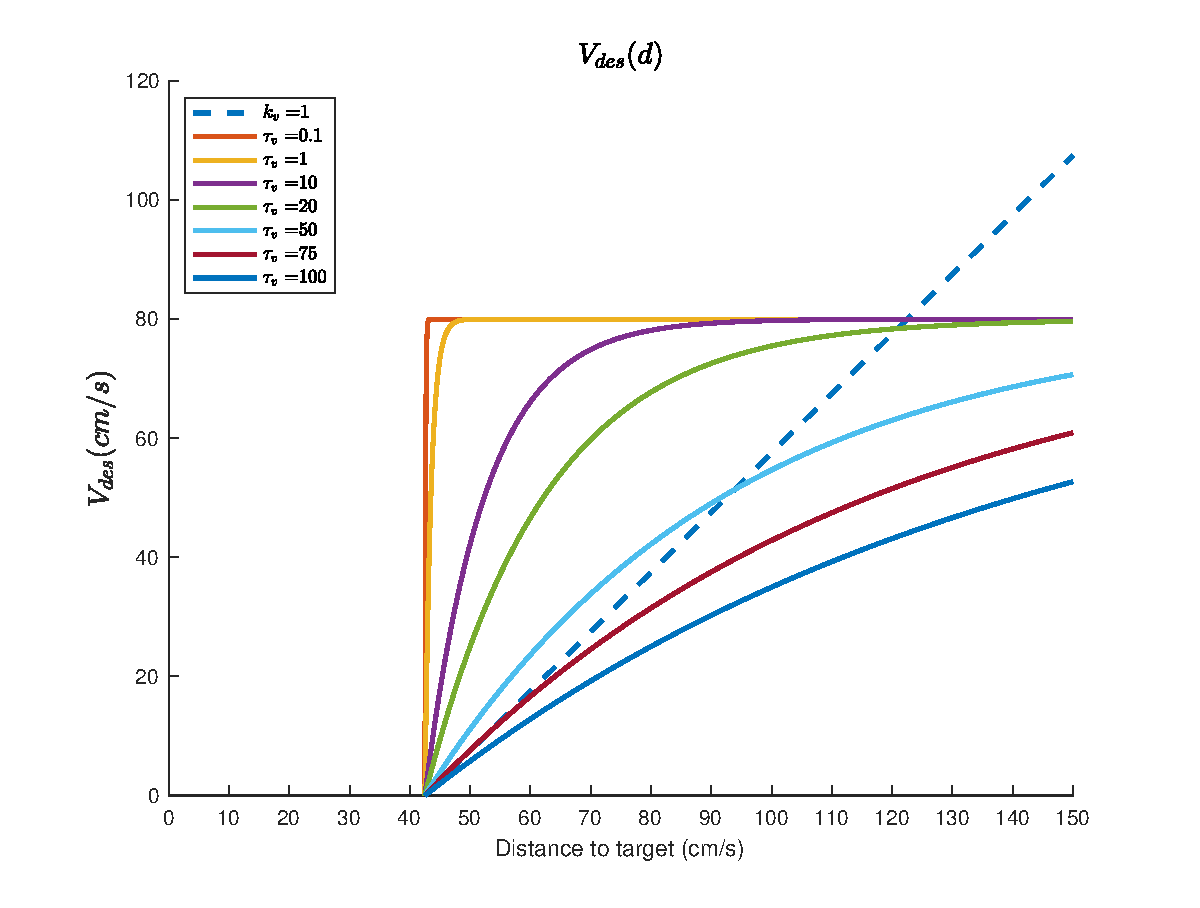
\includegraphics[width=0.7\textwidth]{./img/linear-vel-funcs-comparison-shift.eps}
  \caption{Target acquisition behavior: comparison of functions $v_{des} (d)$
    (with minimum distance shift)}%
\label{fig:linear-vel-funcs-comparison-shift}
\end{figure}
%
%where $k_v$ is the velocity gain with the distance to the target, with $k_v > 0$
%for velocity increase with the distance.

%For this purpose the exponential was chosen has indicated in
%Eq.~(\ref{eq:14}):
%\begin{equation}
%  \label{eq:14}
%  v_{des} (d) = v_{0} \exp(\beta_v d)
%\end{equation}
%where $v_0$ is the velocity near the target (minimum) and $\beta_v$ defines the
%growing rate of the desired velocity as the distance increases.
%

The vector field for linear velocity was implemented (see
(Listing~\ref{lst:program-dyn-tar-vel})) and the parameters were tuned. 
The desired behavior for the robot is faster orientation to target, i.e.,
heading direction dynamics takes precedence over velocity
dynamics. Additionally, the $v_{des}(d)$ must have a slower influence on the
velocity dynamics (smoother curve) to avoid steep accelerations.
Thus, the hierarchy of time constants for the system is: $\tau_{tar} \ll \tau_{v}
\ll \tau_{vdes}$.
% program_dyn_tar.m (generic)
\lstinputlisting[language=matlab, firstline=1,lastline=43,
caption={Implementation of target acquisition behavior with dynamic field for
  linear velocity},label=lst:program-dyn-tar-vel,
style=custom-matlab]{./listing/program_dyn_tar_vel.m}%

The heading direction and velocity dynamics were also plotted, alongside with
$v_{des}(d)$ (see Listing~\ref{lst:program-dyn-tar-vel2}) to aid the behavior analysis.
\lstinputlisting[language=matlab, firstline=89,lastline=141,
caption={Implementation of target acquisition behavior with dynamic field for
  linear velocity},label=lst:program-dyn-tar-vel2,
style=custom-matlab]{./listing/program_dyn_tar_vel.m}%

Fig.~\ref{fig:tar-linear-vel-arena} illustrates the simulation in CoppeliaSim
for the linear velocity dynamics implementation (see also Video
\href{run:./videos/tar-2-3-linear-vel.mp4}{./videos/tar-2-3-linear-vel.mp4}). It can be seen that the robot
successfully moves to target, remaining at a minimum distance. The turning
radius is small, as the heading dynamics has a stronger effect over the robot
than the velocity dynamics. Additionally, during this simulation it was noted
the robot accelerates in the beginning to $1/3$ of the overall distance
$g_{tar}(v) > 0$ and decelerates until it reaches the target (within the minimum
distance). The final state of the simulation is illustrated for $v_{des}(d)$ and
$g_{tar}(v)$ in Figs.~\ref{fig:tar-2-3-vdes} and~\ref{fig:tar-2-3-g-v}. It can
be seen that the desired velocity reaches $0$ m/s and the corresponding dynamics
$g_{tar}(v)$ is near the attractor in deceleration, as expected.
%
\begin{figure}[!hbt]
\centering
    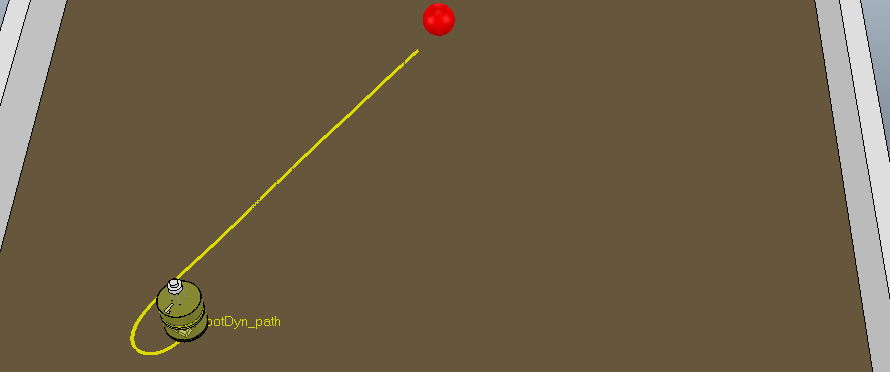
\includegraphics[width=0.7\textwidth]{./img/tar-2-3-arena.png}
  \caption{Target acquisition behavior: velocity dynamics simulation in CoppeliaSim}%
\label{fig:tar-linear-vel-arena}
\end{figure}
%
\begin{figure}[!hbt]
\centering
    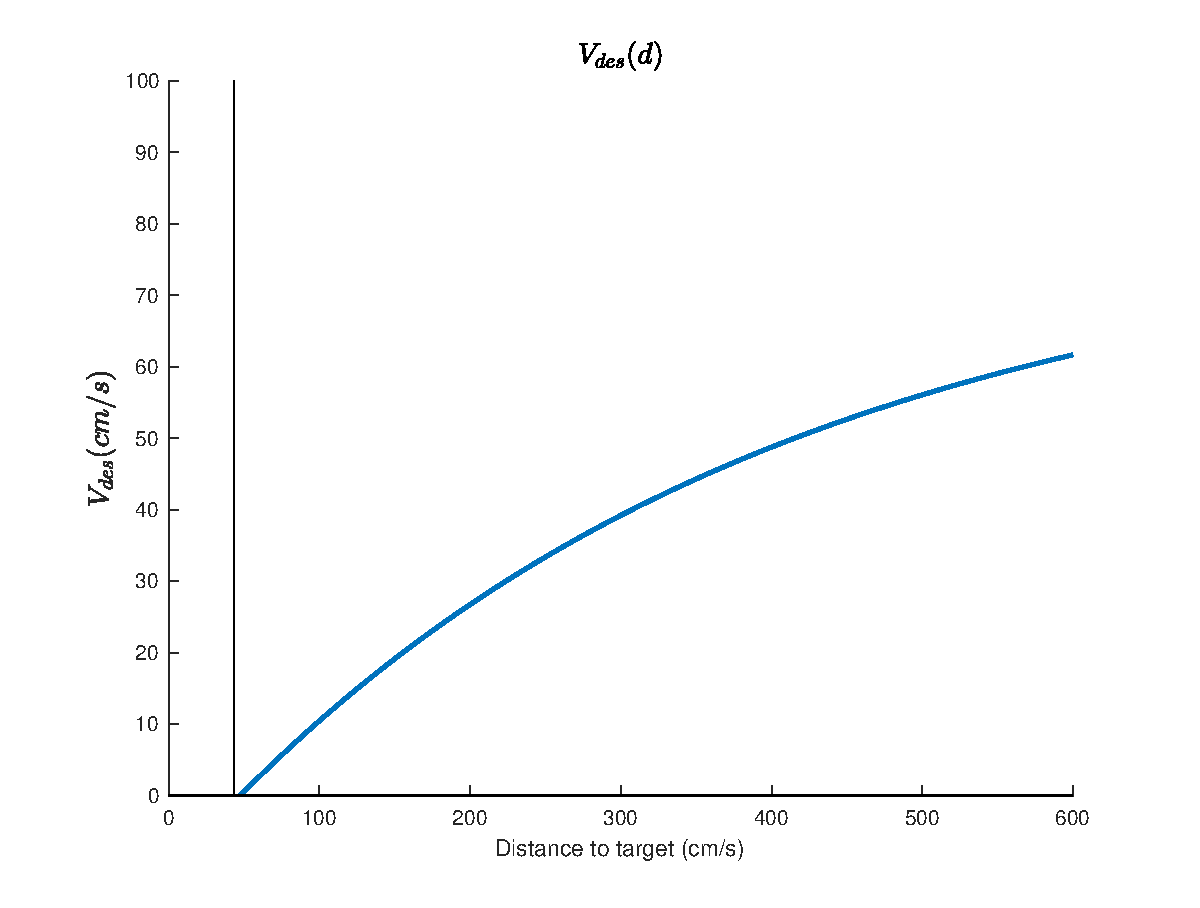
\includegraphics[width=0.7\textwidth]{./img/2-3-vdes.eps}
    \caption{Target acquisition behavior: velocity dynamics simulation ---
      $v_{des} (d)$}%
\label{fig:tar-2-3-vdes}
\end{figure}
%
\begin{figure}[!hbt]
\centering
    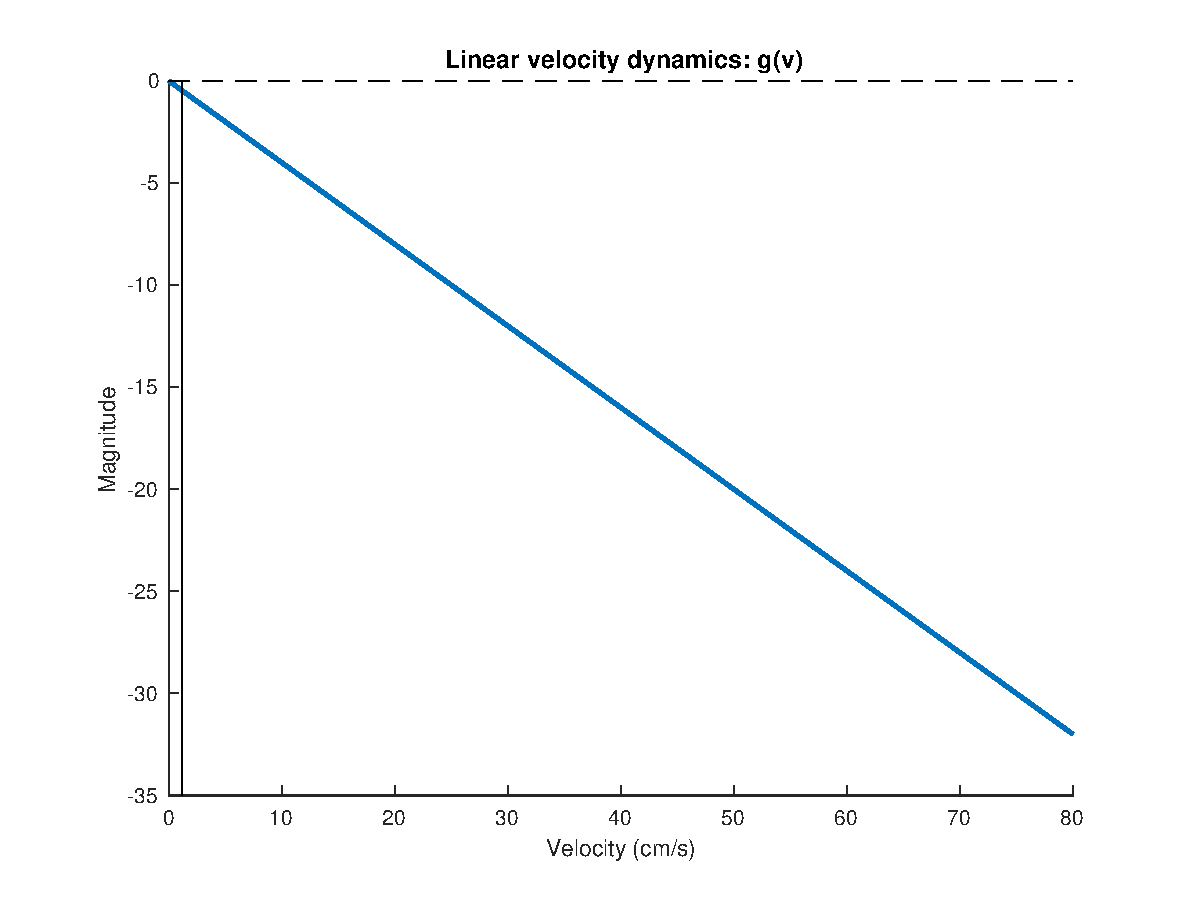
\includegraphics[width=0.7\textwidth]{./img/2-3-g-v.eps}
  \caption{Target acquisition behavior: velocity dynamics simulation ---
    $g_{tar} (v)$}%
\label{fig:tar-2-3-g-v}
\end{figure}
%
\section{Discussion}%
\label{sec:discussion-tar-nonl}
As aforementioned (See Section~\ref{sec:robot-moving-vect-field}), the robot
moves to the target with variable velocity: it accelerates in the beginning to
$1/3$ of the overall distance $g_{tar}(v) > 0$ and decelerates until it reaches
the target (within the minimum distance).
The heading direction dynamics takes precedence
over the velocity dynamics to allow smooth navigation to the target: the robot
orientates itself faster to the target than it actually moves. 
Additionally, the $v_{des}(d)$ has a slower influence on the
velocity dynamics (smoother curve) to avoid steep accelerations.
Thus, the hierarchy of time constants for the system is: $\tau_{tar} \ll \tau_{v}
\ll \tau_{vdes}$.
The heading direction dynamics is illustrated in Fig.~\ref{fig:tar-2-1} and
in Figs.~\ref{fig:tar-2-3-vdes} and~\ref{fig:tar-2-3-g-v} can
be seen that the desired velocity reaches $0$ m/s and the corresponding dynamics
$g_{tar}(v)$ is near the attractor in deceleration, as expected.

\section{Linear dynamic system for heading direction}%
\label{sec:line-dynam-syst}
In this section a linear dynamic system for the heading direction was analyzed:
\begin{equation}
  \label{eq:19}
  \frac{d \phi}{dt} = f_{tar}(\phi) = - \lambda_{tar}(\phi - \psi_{tar})
\end{equation}

The fixed points and its stability was determined. The phase portraits
were plotted and compared to the nonlinear counterpart. Next, the linear dynamic
system was implemented and simulated, observing some differences of the
navigation paths due to higher angular velocity range. Lastly, the linear and
nonlinear dynamic system were compared, determing the best suited for the task
of target acquisition behavior of the robot.
%
\subsection{Fixed points}%
\label{sec:fixed-points-linear-phi}
The fixed points of the linear dynamic system can be determined as its constant
solutions, i.e.:
\begin{equation}
  \label{eq:20}
\begin{array}{ll}
  \left. \frac{d \phi}{dt}\right|_{\phi = \phi^*} = f_{tar}(\phi^*) = 0 \quad 
  \leftrightarrow \quad - \lambda_{tar} (\phi^* - \psi_{tar}) = 0\\
      \quad \leftrightarrow \quad 
  (\lambda_{tar} = 0 \vee \phi^* - \psi_{tar} = 0) \wedge \lambda_{tar} \ne 0
  \quad \leftrightarrow \quad \boxed{\phi^* = \psi_{tar}} \\
\end{array} 
\end{equation}
%
There is one fixed point at $\phi^* = \psi_{tar}$.
%
\subsection{Stability}%
\label{sec:stability-linear-phi}
The determination of the stability of fixed points is useful to understand its
qualitative behavior. It can be determined analytically using Eq.~(\ref{eq:21}):
%
\begin{equation}
  \label{eq:21}
  m = \left. \frac{d f_{tar}(\phi)}{d \phi}\right|_{\phi = \phi^*} = f'_{tar}(\phi^*)
  \quad \leftrightarrow \quad  \boxed{m = - \lambda_{tar}}\\
\end{equation}

Analyzing the possible cases for the slope at the fixed points, it can be
observed that:
\begin{equation}
  \label{eq:22}
  m = \left\{
\begin{array}{ll}
      < 0 , & \lambda_{tar} > 0 \quad \rightarrow \quad \mathrm{attractor} \\
      > 0 , & \lambda_{tar} < 0 \quad \rightarrow \quad \mathrm{repeller} \\
      = 0 , & \lambda_{tar} = 0 \quad \rightarrow \quad \mathrm{inconclusive} \\
\end{array} 
\right. 
\end{equation}
The desired heading direction dynamics requires that an attractor is placed in
the target direction, i.e. $\phi^* = \psi_{tar}$ is an attractor, thus
$\lambda_{tar} > 0$. The relaxation time for the attractor is given by:
\begin{equation}
  \label{eq:23}
 \tau_{tar} = \frac{1}{| f'_{tar}(\phi^*) |} \quad \leftrightarrow \quad \boxed{\tau_{tar} = \frac{1}{\lambda_{tar}}}
\end{equation}
%
\subsection{Phase portraits}%
\label{sec:phase-portraits-1}
Fig.~\ref{fig:tar-4-3} illustrates the different phase portraits for the linear
dynamic system of the heading direction $\phi \in [0, 2 \pi[$ (circular phase
space). Comparing the phase portraits between linear and nonlinear dynamic
systems, respectively Figs.~\ref{fig:tar-4-3} and~\ref{fig:1-3-phase-portraits},
it can be observed that the former has one fixed point only --- 
attractor or repeller depending on the value of the parameter $\lambda_{tar}$,
but not both on the same phase portrait --- while the latter has two fixed
points --- one attractor and one repeller on each phase portrait.
%
\begin{figure}[!hbt]
\centering
    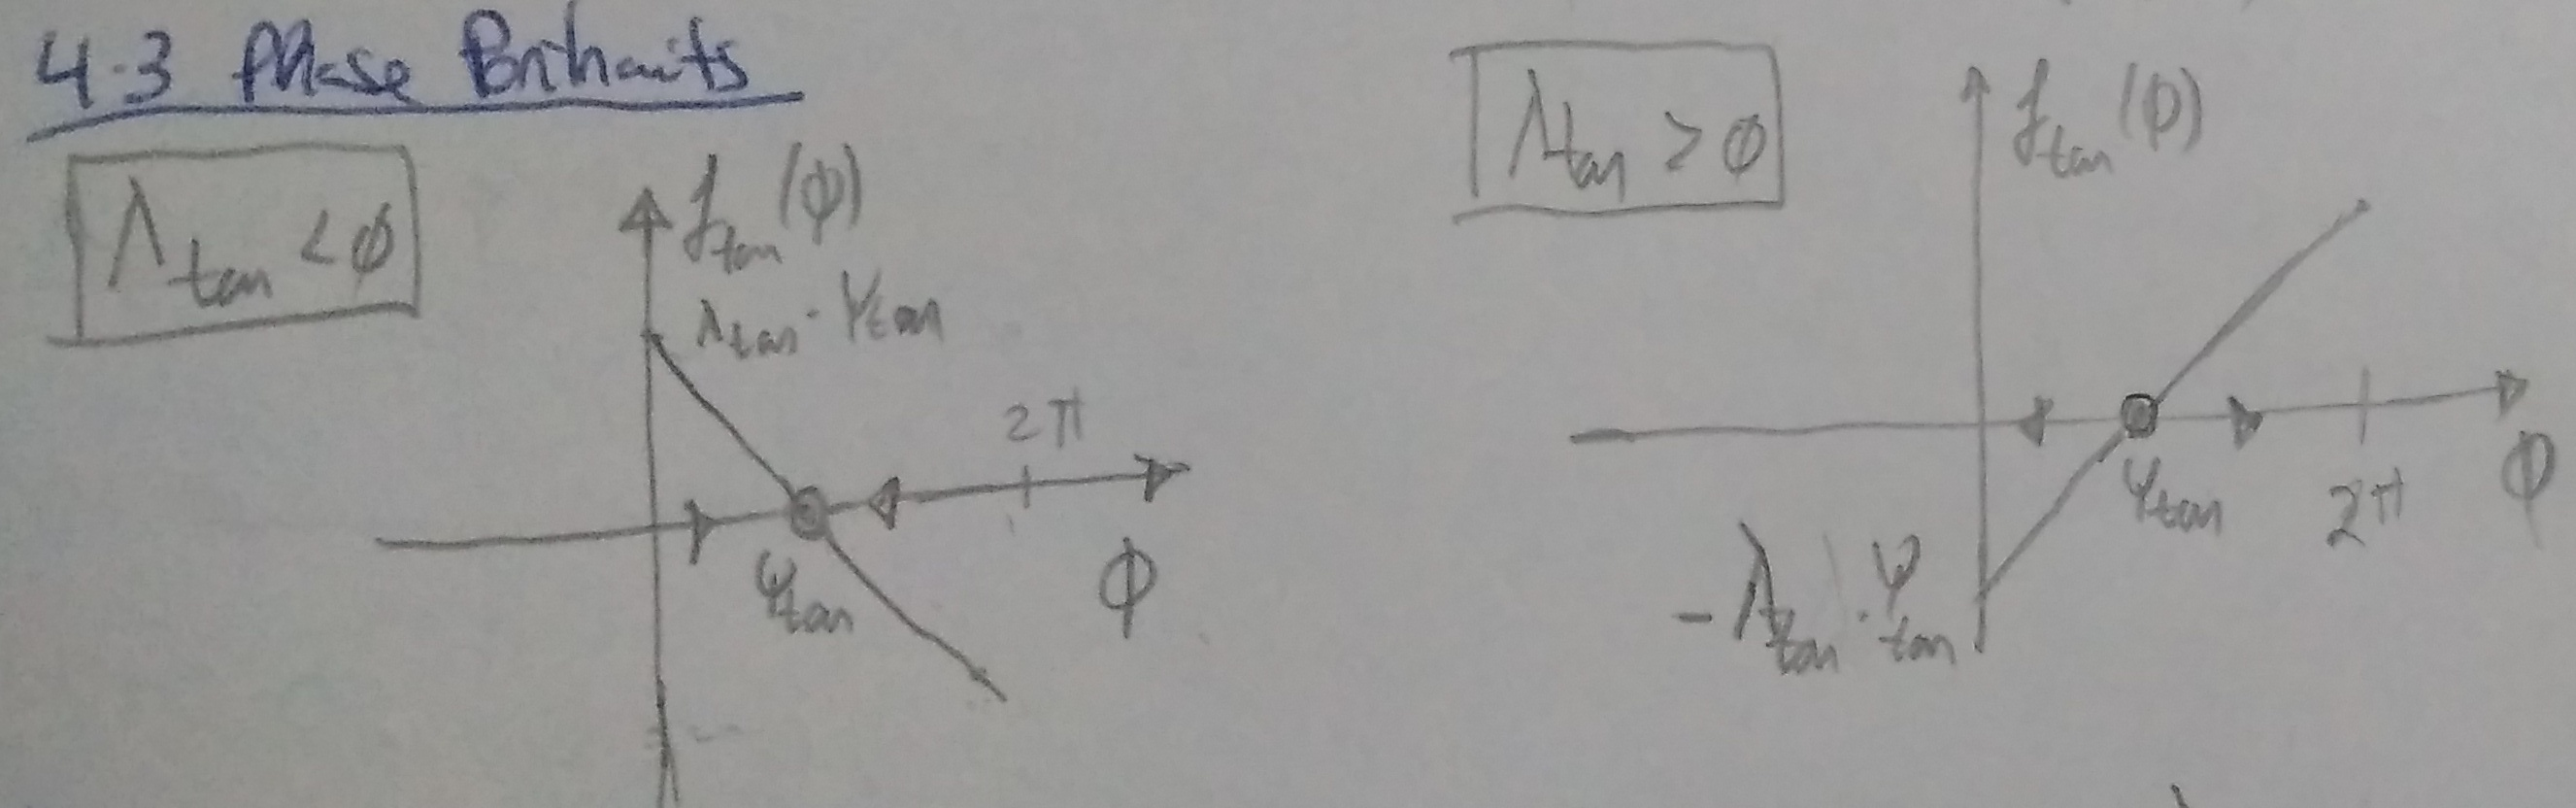
\includegraphics[width=0.8\textwidth]{./img/tar-4-3.jpg}
  \caption{Target acquisition behavior: linear dynamic system for heading
    direction --- phase portraits}%
\label{fig:tar-4-3}
\end{figure}
%
%
\subsection{Implementation}%
\label{sec:implementation-linear-phi}
The implementation of the linear dynamic system for the heading direction was
performed considering also the linear dynamic system for linear velocity, i.e.,
modifying the implementation from Section~\ref{sec:robot-moving-vect-field} with
respect to the heading direction dynamics as follows: 
%
\begin{lstlisting}[language=matlab, caption={Implementation of linear dynamic
system for heading direction},label=lst:program-dyn-tar-linear-phi,
style=custom-matlab]%

% dynamic system
ftar = -lambda_tar * (phirobot - psi_tar);
% plot
ftar_plot = -lambda_tar * (phi_plot - psi_tar);

\end{lstlisting}

The same considerations, in respect to the nonlinear dynamic system, needed to
be applied, namely $\Delta t \ll \tau_{tar}$.

\subsection{Discussion}%
\label{sec:discussion-linear-phi}
Fig.~\ref{fig:tar-4-4-arena} illustrates the simulation of the linear dynamic
system for heading direction implemented (see also \href{run:./videos/tar-4-4.mp4}{./videos/tar-4-4.mp4}), and Fig.~\ref{fig:tar-4-4} contains
the final state of the dynamics. Comparing Fig.~\ref{fig:tar-4-4-arena} with
Fig.~\ref{fig:tar-linear-vel-arena}, respectively the simulation of linear and
nonlinear dynamics, it can be observed the smaller curvature radius
corresponding to the initial orientation to the target for the former. This is
due to the higher magnitude of the attractive force-let (linear) (higher angular
velocity) for linear dynamics, as compared to
the repulsive and attractive force-lets (sinusoidal) for nonlinear
dynamics. The nonlinear dynamic system is better suited for target acquisition
behavior of the robot, as it provides smoother paths --- narrower angular
velocity range.
%
\begin{figure}[!hbt]
\centering
    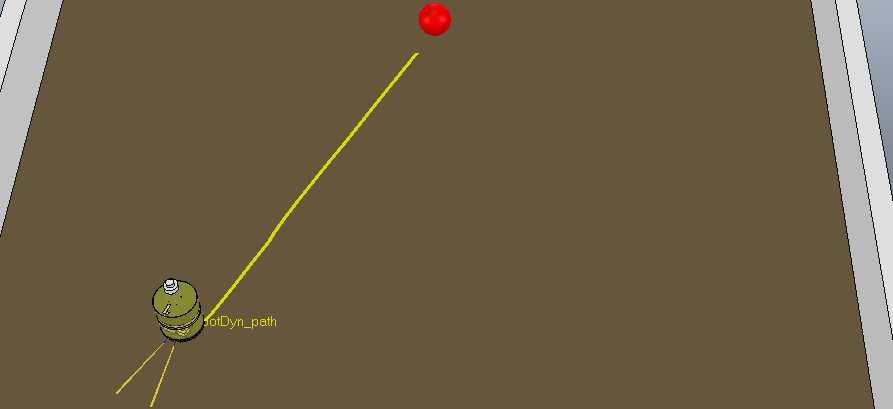
\includegraphics[width=0.65\textwidth]{./img/tar-4-4-arena.png}
  \caption{Target acquisition behavior: linear dynamic system for heading
    direction --- simulation}%
\label{fig:tar-4-4-arena}
\end{figure}
%
\begin{figure}[!hbt]
\centering
    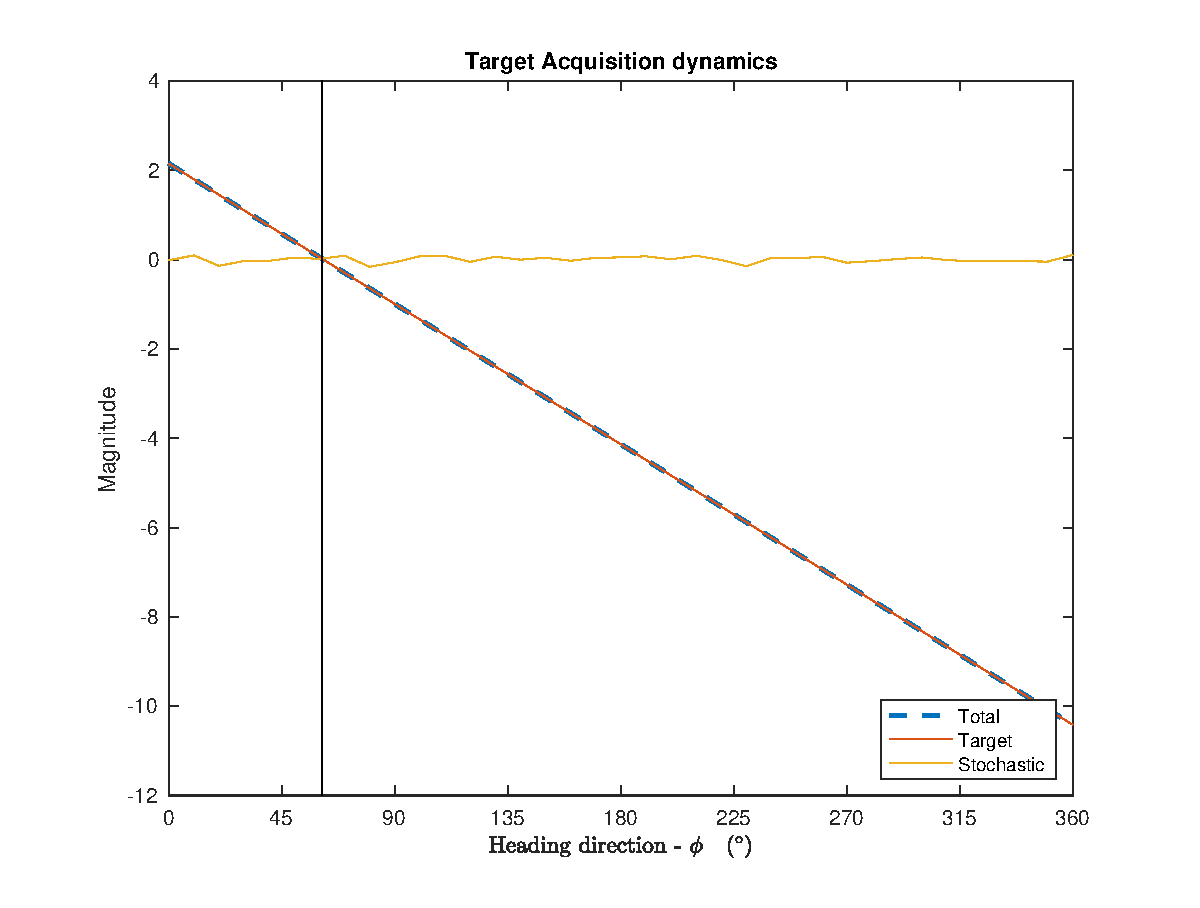
\includegraphics[width=0.65\textwidth]{./img/tar-4-4.eps}
  \caption{Target acquisition behavior: linear dynamic system for heading
    direction --- dynamics (final state)}%
\label{fig:tar-4-4}
\end{figure}
%
%
%
%%% Local Variables:
%%% mode: latex
%%% TeX-master: "../../dissertation"
%%% End:
